\chapter{Estado de la Cuestión}
\label{cap:estadoDeLaCuestion}

Este capítulo lo dedicaremos a estudiar el contexto sobre el que se sustenta nuestro trabajo. Antes de comenzar debemos conocer los trabajos previos que se han realizado en el campo de la navegación y cómo se han abordado desde el punto de vista tecnológico. Nos interesaremos, especialmente, en aquellos enfocados a la navegación por interiores y, en concreto, aquellos cuyo usuario final es una persona con discapacidad visual. 

En la Sección \ref{sec:appGuia} se exponen distintas aplicaciones de navegación. De ellas extraemos sus puntos más fuertes y, sobre todo, sus carencias, pues serán esos puntos donde nuestro trabajo tratará de incidir en mayor medida. En la Sección \ref{sec:sisPos} veremos la tecnología necesaria para el posicionamiento, comparando las tres principales vertientes: GPS, Wi-Fi y Bluetooth. 

\section{Aplicaciones de guía}
\label{sec:appGuia}
En los últimos años ha aumentado la sensibilización tecnológica en áreas como la inclusión de usuarios con discapacidad visual. Es por ello que las tecnologías accesibles tienen, cada vez más, un papel central en el desarrollo de aplicaciones, logrando que estas se abran a un público más amplio.

Al igual que las personas videntes, las personas con ceguera son usuarios de aplicaciones de muy variada índole. Debido a esto, encontramos apps ya adaptadas en categorías como: redes sociales, entretenimiento, lectura, identificación de colores y objetos, etc. 

En esta sección, haremos un pequeño estudio sobre las aplicaciones accesibles existentes en el campo de la navegación, bien sea por interiores o exteriores, y su funcionamiento.
	%PRIMERA App
\subsection{Google Maps}
El pasado 10 de Octubre de 2019, en el ``World Sight Day'', Google dió a conocer la última actualización de la famosa aplicación \textit{Google Maps}\footnote{\url{https://blog.google/products/maps/better-maps-for-people-with-vision-impairments/}}. Esta incluiría una nueva característica desarrollada desde cero por y para personas con discapacidad visual que convertiría a la misma en una app accesible.

El proyecto consiste en la implementación de una nueva funcionalidad que facilita la posibilidad de recibir instrucciones de voz más detalladas y nuevos tipos de anuncios verbales muy útiles para las rutas a pie para personas con visibilidad reducida. Algunas de las nuevas instrucciones incluidas son: informar de manera proactiva que estás en la ruta correcta, la distancia hasta el próximo giro, la dirección en la que estás caminando, avisos para cruzar con precaución si te aproximas a una gran intersección, notificaciones en caso de ser redirigido por causa de haber abandonado accidentalmente la ruta correcta, etc. De esta manera, la aplicación pretende hacer más independientes a las personas con discapacidad visual tratando de que se sientan cómodas y seguras a la hora de explorar lugares nuevos y desconocidos. La guía de voz detallada para la navegación está actualmente en desarrollo para diversos idiomas, estando ya disponible en inglés en los Estados Unidos y en japonés en Japón. Su soporte para otros idiomas y países está en desarrollo.

En cuanto a la navegación por interiores, \textit{Google Maps}\footnote{\url{https://www.google.es/intl/es/maps/about/partners/indoormaps/}} con su actualización $6.0$ incorporó los primeros planos de ciertos edificios públicos, entre los cuales destacan aeropuertos, centros comerciales, estadios y puntos de transporte público. Gracias a esta nueva versión denominada \textit{Google Maps Indoors}, \textit{Google Maps} ayuda a determinar dónde estás, en qué planta y hacia dónde ir. Para ello, basta con hacer \textit{zoom} sobre un edificio cuyo plano esté disponible en la app, y este aparecerá automáticamente y completamente detallado. En la Figuras \ref{fig:ejemplo} y \ref{fig:ejemplo2} vemos un ejemplo del famoso Madison Square Garden de Nueva York.


 

\begin{figure}[t]
	\centering
	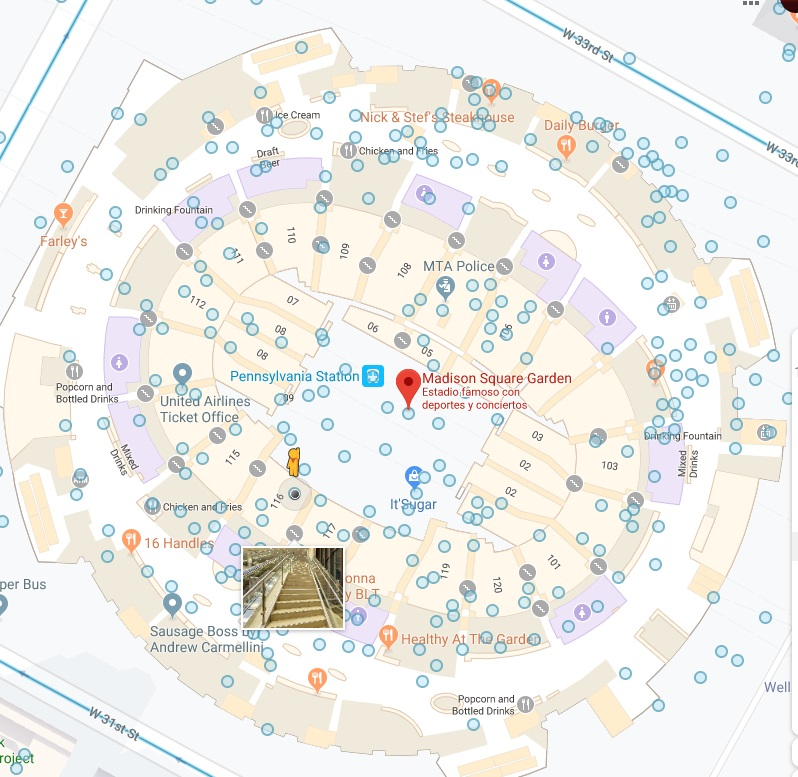
\includegraphics[width=0.6\textwidth]{Imagenes/Estadodelacuestion/MadSq2}
	\caption{Plano de un edificio proporcionado por Google Maps.}
	\label{fig:ejemplo}
\end{figure}

\begin{figure}[t]
	\centering
	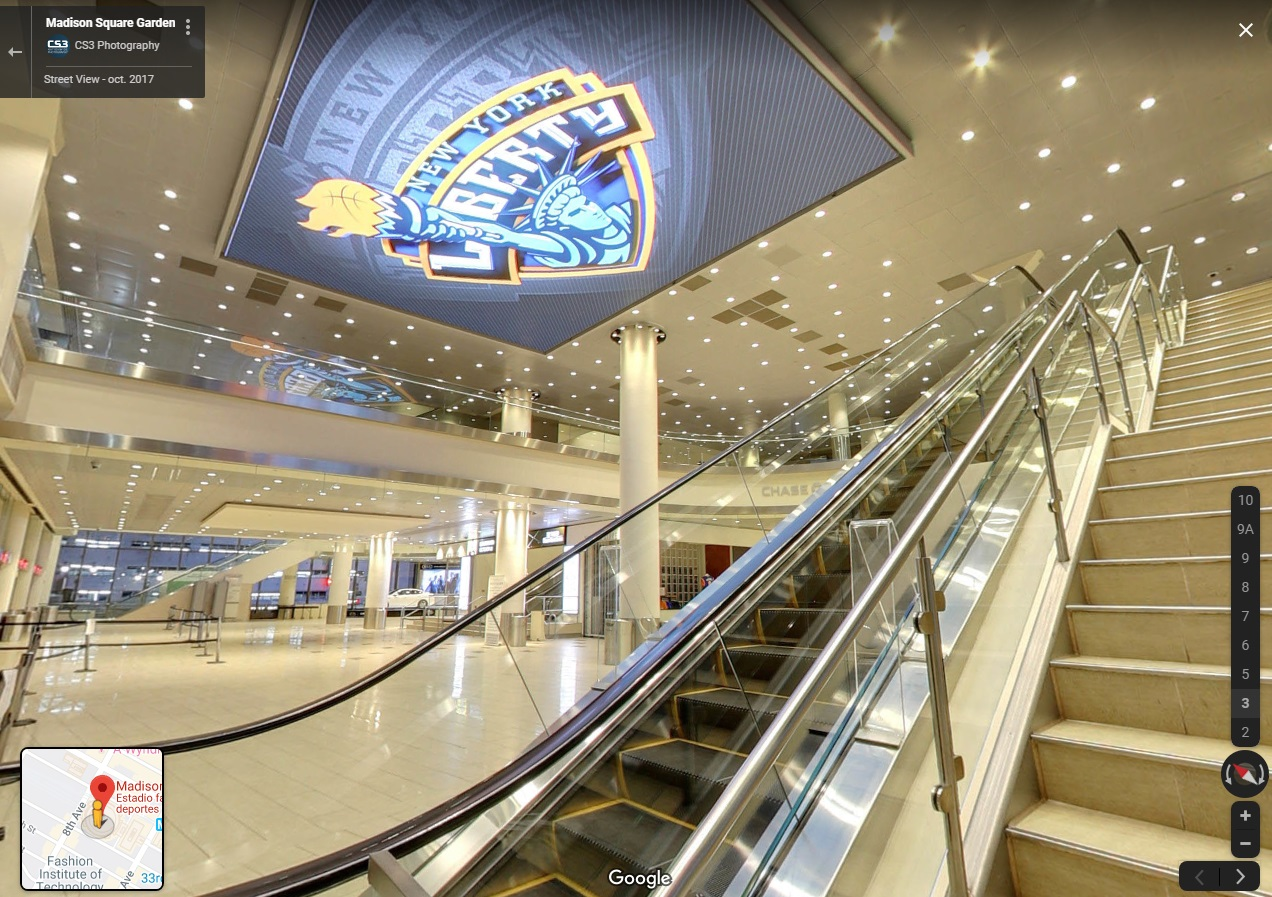
\includegraphics[width=0.6\textwidth]{Imagenes/Estadodelacuestion/MadSq3}
	\caption{Vista del interior del Madison Square Garden. }
	\label{fig:ejemplo2}
\end{figure}

Con estos nuevos planos podrás localizar dónde están los baños, escaleras, ascensores, entradas y salidas, etc., los cuales aparecen representados mediante iconos globalmente aceptados (ver Figura \ref{fig:ejemplo}). También aparecen detallados los distintos establecimientos que se localizan en el edificio e incluye la posibilidad de hacer ciertas búsquedas, tanto generales (de cafeterías, librerías, tiendas, restaurantes...) como concretas (Starbucks, McDonald's...) (ver Figura \ref{fig:ejemplo3}). Otra funcionalidad que no falta en la versión de interiores es la posibilidad de señalar un destino y recibir indicaciones sobre cómo llegar a él. Para ello, aparece el habitual punto azul que te acompaña e indica tu posición, actualizando el plano con cada movimiento que lleves a cabo e incluyendo cambios de una planta a otra (ver Figura \ref{fig:ejemplo3}). Esta aplicación es un proyecto colaborativo y por ende, desde la web es posible actualizar y subir nuevos planos. Está disponible tanto para ordenador como plataformas Android e iOS.

\begin{figure}[t]
	\centering
	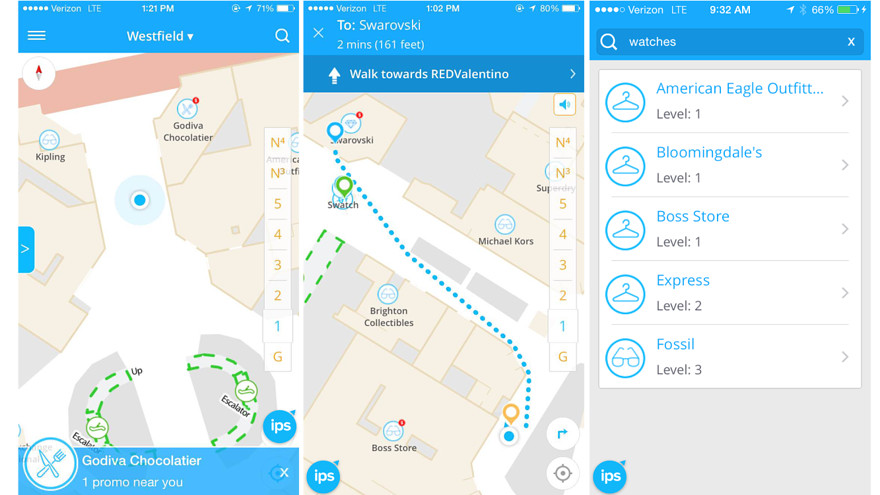
\includegraphics[width=0.6\textwidth]{Imagenes/Estadodelacuestion/GMapsInd}
	\caption{Ejemplo de navegación y búsqueda en Google Maps Indoors. }
	\label{fig:ejemplo3}
\end{figure}

Sin dudar del gran avance que esta aplicación supone en la navegación por interiores, no debemos olvidar algunas de sus desventajas: el posicionamiento, al contrario que en exteriores, no es muy preciso (en la web hablan de varios metros), y las búsquedas que puedes realizar son limitadas, no pudiendo, por ejemplo, preguntar por la ubicación de los baños; esto es, puedes ver dónde están pero no puedes seleccionarlos como destino para que te vaya indicando la ruta a seguir. Pero sobre todo, tiene el inconveniente de que no es una tecnología accesible: \textit{Google Maps Indoors}\footnote{\url{https://www.youtube.com/watch?v=cPsTWj_O3Qs}} es una aplicación completamente visual que no cuenta con soporte auditivo por lo que descarta completamente a usuarios invidentes.



%SEGUNDA APP
\subsection{BlindSquare}
\textit{BlindSquare}\footnote{\url{https://www.blindsquare.com}} es una de las aplicaciones de navegación más populares. Su uso se extiende a más de 130 países y está disponible en 25 idiomas, entre los cuales se incluye el español. Esta aplicación, desarrollada para iOS y diseñada para personas con discapacidad visual, proporciona una guía completa, de origen a destino, tanto en exteriores como en interiores. Además, describe el entorno y anuncia posibles puntos de interés para el usuario (como pueden ser los lugares considerados populares o aquellos visitados frecuentemente). Su principal característica es que permite interactuar mediante voz gracias al controlador de música de Apple. 

Esta aplicación determina tu posición mediante localización \textit{GPS} y, a partir de ahí, puede darte información sobre las proximidades utilizando \textit{Foursquare} y \textit{OpenStreetMap}. De este modo, es capaz tanto de guiarte a un cierto destino como de notificarte qué establecimientos hay en tu radio: restaurantes a 200m, parques más cercanos, farmacias...

Con el fin de agilizar el uso de la app, y que por tanto esta sea cómoda y rentable para los usuarios finales, incluye: accesos directos a funciones mediante gestos (como sacudir el móvil para que nos diga la ubicación actual y puntos cercanos) y la posibilidad de establecer filtros para recibir únicamente el tipo de información deseada. Por ejemplo, permite filtrar por restaurantes para no tener notificaciones sobre estaciones de tren o librerías.

En cuanto a la navegación por interiores, \textit{BlindSquare}\footnote{\url{https://www.youtube.com/watch?v=9jH-Bdjmgb4}} emplea un sistema de balizas Bluetooth, también llamadas \textit{beacons}, que colocan en sitios estratégicos de los edificios, para solventar el problema del posicionamiento. Por lo demás, incluye las mismas posibilidades y funcionalidades que la navegación por exteriores, con la única limitación de que el edificio debe estar provisto de dichos sistemas de posicionamiento.

En su web encontramos un ejemplo de la utilización de los \textit{beacons} en un campus\footnote{\url{https://www.blindsquare.com/2019/11/01/blindsquares-getting-straight-as-on-campus/}}: una vez que entras en el edificio, uno de los \textit{beacons} reconocerá tu aplicación \textit{BlindSquare} y te hará saber dónde te encuentras y cómo llegar a tu destino, indicándote los ascensores, escaleras e intersecciones más cercanas. Integrar en el campus servicios como estos favorece tanto a visitantes como a estudiantes con discapacidad visual moverse por el entorno con total autonomía y seguridad.

A modo de resumen, entre los puntos fuertes de esta aplicación destacamos los siguientes:
\begin{itemize}
	\item Da información sobre los metros que quedan hasta llegar a un determinado objetivo. Resulta útil porque si van disminuyendo sabes que vas por el camino adecuado.
	
	\item Utiliza indicaciones de tipo reloj (a las 10, a las 3,...) muy usadas por las personas con discapacidad visual\footnote{\url{http://www.riate.org/version/v1/materiales_en_prueba/e_inclusiva_discapacidad/pdf/m6_dv.pdf}}.
	
	\item Avisa de las intersecciones. 
	
	\item Cuando se supera una nueva indicación, la aplicación emite el sonido asociado a correto o \textit{check}. En el caso de que la indicación no sea completada correctamente, se reproduce otro sonido en consecuencia.
	
	\item Se pueden añadir ubicaciones en una lista de lugares marcados.
	
	\item Se puede ir girando con el móvil mientras la aplicación indica los puntos de interés que se encuentre delante. 
	
	\item También tiene opción de simulación, que permite prepararse un camino antes de ir.
	
	\item Permite ser más autónomo y descubrir nuevos sitios.
	
	\item En los desplazamientos indica las distintas alternativas por adelantado. Esto es, mientras que para espacios exteriores señala la posible ruta utilizando transporte público, privado, a pie, etc, para espacios interiores especifica, siempre que la haya, la opción de utilizar escaleras, ascensor, escaleras mecánicas, etc. De esta manera proporciona una idea global del espacio y de las distintas vías que se pueden seguir para llegar al destino.
	
	\item Permite llevar las manos libres.
	
	\item Incluye un lector de códigos QR, que es cómodo porque puede dar más información que la línea braille.
\end{itemize}

Su principal punto negativo es el precio, ya que cuesta 40 libras.

Al contrario que la aplicación \textit{Google Maps Indoors}, esta sí es una aplicación diseñada para personas con discapacidad visual. Las diferencias saltan a la vista: el modo de dar las indicaciones, avisos constantes para indicar si se va por el camino correcto, permite más autonomía gracias a la comunicación constante que ofrece permite llevar las manos libres, entre otras cosas. Parece imposible pensar que el interior de un edificio pueda resultar menos seguro que una gran avenida, pero lo cierto es que, para las personas con discapacidad visual, muchas veces es así. El interior de un gran centro comercial o una biblioteca resultan un laberinto cuando se va por primera vez, más aún si tenemos algún tipo de dificultad para leer las indicaciones que, normalmente, suelen estar en lugares altos y no adaptadas para personas con discapacidad visual. Lo que se pretende con esta aplicación es mantener la autonomía del usuario tanto dentro como fuera de un edificio\footnote{\url{https://www.blindsquare.com/2019/10/24/independence-on-both-sides-of-the-door/}}.

\subsection{Nearby Explorer}
\textit{Nearby Explorer}\footnote{\url{https://play.google.com/store/apps/details?id=org.aph.nearbyonline&hl=es}} es otra de las aplicaciones que encuadramos en el campo de la navegación accesible por interiores y exteriores. Está disponible tanto para Android como para iOS y su descarga se encuentra disponible de manera gratuita. 

La guía por exteriores se basa en la misma idea que \textit{BlindSquare}, y por ende funciona de manera similar. Entre sus características destacan: la posibilidad de ejecutar ciertas acciones poniendo el móvil en distintas posiciones, como por ejemplo, inclinarlo verticalmente para que funcione como una brújula y la capacidad de filtrar la información de modo que ésta se adapte completamente a las necesidades del usuario. Entre la información que \textit{Nearby Explorer} puede proporcionar a sus usuarios encontramos los lugares cercanos a la ubicación actual, los nombres de las calles por las que pasa, los números de los bloques de las calles por las que pasa, la distancia que hay al destino desde un punto de referencia (como casa, trabajo...), etc. Además de la posibilidad de filtrar la información deseada, las indicaciones por audio pueden ser pausadas en cualquier momento de modo que no interfieran con otras señales auditivas (como las paradas en un autobús, por ejemplo). Otra gran funcionalidad con la que cuenta \textit{Nearby Explorer} es la de explorar una ruta por adelantado, sin tener que estar físicamente en el sitio, pudiendo incrementar o decrementar el radio de exploración.

Por otro lado, la navegación por interiores se basa en un sistema de \textit{beacons} que sustituye a las señales GPS y se encarga de solventar el problema del posicionamiento en interiores. Pueden configurarse de dos maneras: \textit{ad hoc} y \textit{mapeo completo}.

En el caso de la configuración \textit{ad hoc}, cuenta con la ventaja de que tiene una instalación muy sencilla (basta con posicionar los \textit{beacons} sobre la pared, en la ubicación que queramos)\footnote{\url{https://tech.aph.org/neios/\#Beacon}}, pero aparecen los siguientes problemas:
\begin{itemize}
	\item No se puede determinar la ubicación exacta de un \textit{beacon}.
	\item No se puede obtener información del entorno a menos que te encuentres dentro del radio de detección de un \textit{beacon}.
	\item Tienes que habilitar cierto soporte para detectar los \textit{beacons} (no se detectan de manera automática).
\end{itemize}

Por el contrario, el \textit{mapeo completo} es más robusto por lo que su instalación es más compleja pero a cambio nos proporciona una localización precisa del dispositivo por lo que tiene un comportamiento similar al de otras aplicaciones.

Desde el punto de vista de la navegación por exteriores es una aplicación completa y fácil de utilizar, que incluye una interfaz sencilla y trata de adaptarse siempre a las distintas necesidades o situaciones del usuario mediante opciones configurables. Además, cuenta con una versión gratuita (algo poco común en aplicaciones de tal categoría) que aunque no incluye todas las funcionalidades de la versión de pago te permite probarla y familiarizarte con ella antes de tomar una decisión final. Por otro lado, la funcionalidad de navegación por interiores no está tan desarrollada y su uso está supeditado exclusivamente a aquellos lugares que cuenten con la instalación necesaria y hayan incluido sus datos en OpenStreetMap, configurando el espacio en nodos, aristas y relaciones. Esta tarea es tediosa y a menudo parte de cero por lo que son pocos los edificios que actualmente están mapeados y pueden aprovechar al máximo la app.

\subsection{Lazarillo}
Lazarillo\footnote{\url{https://www.lazarillo.app/es/}} es una aplicación de guía para personas con discapacidad visual que actualmente solo proporciona guía para exteriores. Inicialmente la idea era cubrir también la navegación por interiores pero su desarrollo no fue posible por problemas de financiación.

La navegación por exteriores cuenta con las funcionalidades básicas que ya hemos mencionado en las apps anteriores: \begin{itemize}
	\item Buscar lugares de interés, cercanos a la ubicación actual. Esta búsqueda se puede acotar filtrando por categorías que vienen predefinidas (transporte, bancos y cajeros, salud, comida, tiendas, etc.).
	\item Buscar una dirección específica a partir de la cual se desplegarán todas las posibles rutas (a pie, en transporte público, privado, etc.) y una vez seleccionada la ruta deseada, comenzarán las indicaciones mediante audio con la información pertinente (metros, giros a derecha e izquierda, etc. ). 
	\item Guardar una lista de lugares favoritos.
	\item Posibilidad de rastrear una dirección, previamente marcada con la opción ``Seguir este lugar'', de modo que con independencia de a dónde nos estemos dirigiendo se activará una alerta a medida que nos acerquemos a dicha ubicación.
	\item Ajustar la configuración de las indicaciones, velocidad, tipo de voz...
\end{itemize}

En resumidas cuentas, \textit{Lazarillo} es una aplicación que, como otras, busca mejorar la calidad de vida de las personas con discapacidad visual indicándoles para ello qué les rodea y proporcionándoles una mayor independencia. Ésta, sin embargo, cubre únicamente los aspectos más básicos y elementales sin reparar en otras posibles funcionalidades o indicaciones (obstáculos, peligros...), por lo que es una aplicación incompleta.

La app es completamente gratuita y cuenta con versión para Android y iOs.


\subsection{Wayfindr} 
\textit{Wayfindr}\footnote{\url{https://www.wayfindr.net/}} nació en 2015 en Londres, con la misión de capacitar a las personas con discapacidad visual para que viajen de manera independiente a través de una navegación de audio inclusiva y accesible. Con este fin, han desarrollado el primer estándar del mundo aprobado internacionalmente para la navegación de audio accesible y ya cuentan con las primeras demostraciones de un sistema de navegación en red. Este sistema, basado en audio, pretende dar soporte para que las personas con discapacidad visual puedan adentrarse por esos lugares que están repletos de señales escritas, por los que las personas que ven pasan sin pensar, pero que son precisamente los que más temen y evitan aquellos que tienen discapacidad visual (estaciones de metro, tren, aeropuertos, centros comerciales, hospitales, etc.). 

Este proyecto de código abierto ha realizado ya numerosas pruebas en distintos escenarios, como por ejemplo en el metro de Londres (o, más recientemente, en el metro de Los Ángeles) donde el funcionamiento\footnote{\url{https://www.youtube.com/watch?v=mc3KmbfxuUQ}} de la aplicación es tan práctico como sencillo: se basa en una serie de \textit{beacons}, colocados en puntos estratégicos a lo largo de las distintas estaciones de metro, que emiten unas señales que son captadas por el móvil a su paso por un cierto radio de detección. Estas señales permiten ubicar al usuario y darle la siguiente indicación con el propósito de alcanzar su objetivo (coger un tren o salir de la estación). Los desarrolladores recomiendan el uso de auriculares de conducción ósea, de manera que puedan escuchar otros sonidos del exterior.

La idea de este proyecto supone un gran avance para las personas que tienen algún tipo de discapacidad visual, ya que pretende empoderarlas para que no se sientan retenidas por su pérdida de visión ni tengan que vivir supeditadas a una persona vidente que las ayude, logrando así que se rompan de una vez por todas las barreras a las que están sometidas. Para la consecución de este fin, esta organización sin ánimo de lucro proporciona a los fabricantes de navegación digital y propietarios de espacios públicos las habilidades y técnicas para proporcionar a las personas con discapacidad visual servicios de navegación digital consistentes y de alta calidad. \textit{Wayfindr} utiliza varias tecnologías para rastrear la ubicación de una persona y activar el audio de las instrucciones en su teléfono móvil en el momento adecuado para llevarlos a su destino. De esta manera, busca permitir que las personas con discapacidad visual naveguen por el mundo utilizando las instrucciones de audio de sus teléfonos inteligentes.

%\subsection{Conclusiones}
%Tras este breve recorrido por algunas de las aplicaciones de navegación adaptadas para personas ciegas o con visibilidad reducida podemos decir que cada vez son más las opciones disponibles. Hemos visto desde aplicaciones de navegación por exteriores, como también por interiores, llegando hasta algunas tan específicas como \textit{Wayfindr} que está dirigida al metro de Londres concretamente. Todas ellas se rigen por un patrón común: el de la simpleza, sin conllevar por ello una reducción de la funcionalidad. Estas aplicaciones nos permiten filtrar la información que se quiere recibir, guardar nuestros lugares más visitados, manejarlas mediante voz o con sacudidas del teléfono..., es decir, nos proporcionan un gran abanico de posibilidades que el usuario puede ejecutar de manera sencilla.
%
%Por otro lado, si comparamos las apps, encontramos que aquellas de navegación por interiores están aún por desarrollar ya que el mapeo del interior de los edificios debe realizarse de manera particular e individual, convirtiéndose en una tarea mucho más tediosa que la que lleva a cabo el famoso coche de \textit{Google Maps}. Además, el posicionamiento también es más complejo ya que no es posible utilizar el sistema GPS y hay que recurrir a la triangulación de señales Wi-Fi o a las balizas bluetooth, teniendo que estudiar de nuevo cada caso concreto.


\section{Sistemas de posicionamiento}
\label{sec:sisPos}
Para la consecución de nuestro objetivo, el desarrollo de una aplicación de navegación por interiores, uno de los primeros problemas que se nos plantea es el del posicionamiento en un mapa ya que es de vital importancia poder determinar donde estamos para después indicar la ruta pertinente hacia el destino indicado. En esta sección haremos un pequeño estudio sobre las distintas tecnologías existentes que nos permiten solventar nuestro problema y determinar la posición exacta de un cierto dispositivo, y discutiremos su validez para su aplicación a este Trabajo de Fin de Grado.

\subsection{GPS}

El Sistema de Posicionamiento Global (GPS por sus siglas en inglés) es un sistema de localización diseñado por el Departamento de
Defensa de los Estados Unidos con fines militares para proporcionar estimaciones precisas de posición,
velocidad y tiempo. Este sistema se encuentra operativo desde enero de 1994 y se desarrolló a partir de los 24 satélites que componen la constelación NAVSTAR, cada uno de los cuales cuenta con una órbita de 26.560 Km de radio y un periodo de 12h \citep{pozo2000sistema}. 

El método mediante el cual el GPS determina la altitud, longitud y latitud de cualquier objeto que se encuentre en la superficie terrestre se conoce como triangulación. Este requiere la distancia desde el dispositivo en cuestión (receptor) a tres satélites como mínimo cuya localización es conocida de antemano. Entonces, cuando el receptor detecta el primer satélite, se genera una esfera a su alrededor cuyo radio será la distancia desde el receptor hasta dicho satélite. De este modo, el receptor se encontrará en un punto de la superficie de esa esfera, aún por determinar. Repetimos el proceso con otro satélite. Al crearse esa segunda esfera, el dispositivo receptor se encontrará en alguno de los puntos de corte de ambas esferas, por lo que el resto de puntos se descartan. De nuevo, se utiliza un tercer satélite de modo que se crea una nueva esfera que cortará a las
anteriores. De este modo, con el corte de las tres esferas, y teniendo en cuenta que el dispositivo se encuentra en la superficie terrestre, tendremos el punto concreto buscado. En caso de querer conocer la altitud, bastará con usar un cuarto satélite como referencia y repetir el proceso. En la Figura \ref{fig:ejemplogps} vemos un esquema del proceso que acabamos de explicar empleando 3 y 4 satélites.

El problema del Sistema de Posicionamiento Global es que pierde mucha precisión cuando nos encontramos bajo superficies como túneles, tejados, etc. ya que la señal se debilita enormemente y el dispositivo no es capaz de llevar a cabo la triangulación de manera exacta. Es por esto que descartamos este sistema para nuestro trabajo, que se basa en la guía por interiores.

\begin{figure}[t]
	\centering
	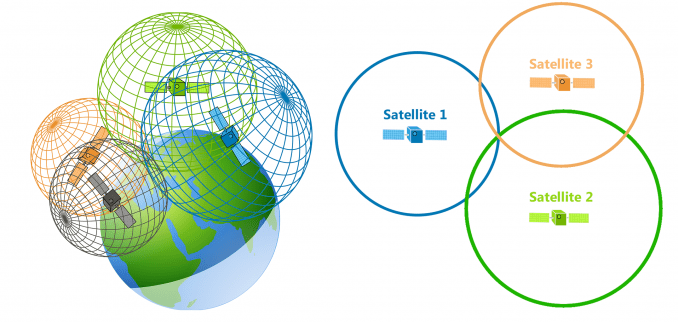
\includegraphics[width=0.6\textwidth]{Imagenes/Estadodelacuestion/triangulacion}
	\caption{Método de triangulación GPS. }
	\label{fig:ejemplogps}
\end{figure}


\subsection{Wi-Fi}

La técnica de posicionamiento mediante señales Wi-Fi fue una de las primeras que surgió para solventar el problema de la localización en interiores. Tal y como hemos mencionado en el apartado anterior, la señal GPS no es suficiente pues las barreras arquitectónicas como las paredes o tejados la debilitan enormemente. Por ello apareció esta técnica que se basa en leer con un dispositivo la intensidad de señal que recibe desde distintos puntos de acceso Wi-Fi del edificio. Una vez leída esta señal existen varios métodos para establecer la posición exacta del dispositivo. El más utilizado se basa en medir la intensidad con la que se recibe la señal en un cierto punto (\textit{Received Signal Strength Indicator, RSSI}) desde varios puntos de acceso y, en base a eso, establecer la localización en la que se encuentra el dispositivo. Este método es fácil y barato de implementar. Su mayor inconveniente es que no proporciona una buena exactitud (de 2 a 5 metros) \citep{wifipositioning}, ya que la señal es muy dependiente del ambiente: personas, paredes, etc.

Otro método que también se utiliza es el denominado \textit{fingerprint}. Este consiste en guardar la intensidad de la señal desde distintos puntos de acceso en una base de datos de acuerdo a coordenadas conocidas del cliente durante una fase sin conexión. Durante la fase de conexión, las medidas actuales RSSI de una posición que no se conoce se comparan con las guardadas en la base de datos y, aquellas que más se le parezcan, se devuelven como estimación de la posición del usuario. Esta técnica tiene mejores resultados en cuanto a la exactitud, cuyo error baja a menos de 3m \citep{wifipositioning}. 

Una de las grandes ventajas de la tecnología Wi-Fi es que prácticamente la totalidad de las casas, colegios y edificios en general están equipados con una red Wi-Fi.


\subsection{Balizas Bluetooth}

Los \textit{beacons} o balizas Bluetooth son pequeños dispositivos que emiten señales de radio. Estas señales los identifican de manera única y pueden ser captadas por otros dispositivos receptores, estableciéndose así un canal de comunicación que permanece vivo siempre que los receptores permanezcan en un radio de alcance de entre 10 y 30 metros como máximo, según el dispositivo. Es importante remarcar que generalmente los \textit{beacons} no aceptan conexiones de otros dispositivos, lo que significa que no pueden registrar qué aparatos están cerca. Por tanto, esta simplicidad conlleva la necesidad de una aplicación capaz de interpretar la señal de la baliza. Otra característica de los \textit{beacons} es que son de bajo consumo, es decir, sus baterías tienen una duración muy prolongada (aproximadamente 2 años) con una simple pila de botón, y su coste es reducido.

Esta tecnología se hizo muy popular en 2013 cuando Apple introdujo el estándar \textit{iBeacon}\footnote{\url{https://developer.apple.com/ibeacon/}} y comenzó a utilizarlos para la navegación, más concretamente, para el posicionamiento en interiores. En 2015 Google, que no quiso quedarse atrás, lanzó el protocolo Eddystone, un protocolo que, a diferencia del de Apple, es de código abierto y ofrece soporte oficial tanto para iOS como para Android. Otra ventaja que incluye la versión de Google es que proporciona dos APIs que facilitan mucho el manejo de los \textit{beacons}, y que emite cuatro paquetes distintos de información\footnote{\url{https://developers.google.com/beacons/eddystone}}, en lugar de uno como en el caso de los \textit{iBeacons}. Estos paquetes son:

\begin{itemize}
	\item \textbf{Eddystone-UID:} transmite un identificador de baliza único compuesto por 16 bytes, 10 de ellos referidos al espacio de nombres, que identifican a un grupo de \textit{beacons}, y 6 que se refieren e identifican a la instancia particular dentro del grupo. Esta distinción entre espacio de nombres e instancia se pensó para optimizar el escaneo de \textit{beacons}. Este paquete es idéntico al que ofrecen los \textit{iBeacons}.
	
	\item \textbf{Eddystone-URL:} transmite una URL, utilizando un formato de codificación, que se muestra como notificación silenciosa en el dispositivo.
	
	\item \textbf{Eddystone-TLM:} transmite información sobre la baliza: el nivel de la batería, los datos del sensor u otra información relevante para los administradores de balizas. Para poder usarse también como baliza necesita ir acompañado de otro tipo de marco (Eddystone-URL o Eddystone-UID).
	
	\item \textbf{Eddystone-EID:} emite un identificador encriptado que cambia periódicamente, de modo que su uso está restringido a aplicaciones y dispositivos autorizados.
\end{itemize}

Por todo esto, consideramos que utilizar el protocolo Eddystone es más ventajoso para nuestra aplicación, debido a la comodidad y facilidad que nos proporcionan las APIs 

Por otro lado, de cara a establecer la posición exacta de un dispositivo receptor hay dos alternativas, una de ellas es triangular la posición a partir de la distancia obtenida por la señal de los tres \textit{beacons} más cercanos. El inconveniente de este método es que se requiere un número muy alto de balizas para poder cubrir por completo todo el espacio, por lo que los costes de la instalación se elevan. Además, cualquier cambio en la estructura del edificio puede afectar a la posición de los \textit{beacons} y, por ende, al algoritmo de triangulación. El otro método consiste en establecer los \textit{beacons} en puntos de decisión (\textit{landmarks}) donde los usuarios esperan recibir instrucciones. Algunos de estos puntos son las puertas, escaleras, intersecciones, etc. El número de balizas necesario es mucho más reducido por lo que los costes derivados de la instalación también. No obstante, hay que tener en cuenta que es muy importante decidir con cuidado la disposición exacta de los \textit{beacons} para que estén lo menos expuestos posible a interferencias. 

\subsubsection{Interferencias en la señal Bluetooth}
\label{sec:Interferencias}
Los \textit{beacons} son dispositivos que se pueden colocar tanto en interiores como en exteriores pero hay que tener en cuenta qué lugares son más aptos para su establecimiento de manera que la señal no sufra interferencias. Algunas recomendaciones son:
\begin{itemize}
	\item Lugares altos (alrededor de 2,5m) para evitar las interferencias provocadas por los cuerpos de las personas ya que estos absorben parte de la señal.
	\item Lugares alejados a un metro aproximadamente de elementos que pueden alterar la intensidad de la señal como elementos metálicos, conductos de electricidad, iluminación, otras balizas, etc.
	\item En pasillos de menos de 4m de ancho, colocar la baliza en el centro para que cubra el espacio por igual. Si por el contrario el ancho es mayor, se deberán usar varias balizas.
	\item Colocar las balizas aproximadamente 1m antes de los lugares de interés (\textit{landmarks}). Ejemplo: puertas, ascensores, escaleras, esquinas, etc.
	\item Considerar la orientación adecuada de la antena direccional del \textit{beacon}, aunque esta depende por completo del fabricante. En ocasiones la baliza no emite una señal simétrica por completo sino que emite una señal en forma elíptica.
\end{itemize}

Otros factores difíciles de controlar que también afectan a la señal son las condiciones meteorológicas, la señal Wi-Fi, las señales Bluetooth de otros dispositivos \citep{beaconsinterferences}...


\section{Trabajos previos}
\label{sec:trabajos_previos}

Además del estudio de las aplicaciones ya existentes y de las distintas opciones para resolver el problema del posicionamiento, es importante conocer algunos de los trabajos previos que se han hecho en el campo de la navegación por interiores. En concreto nos centramos en dos Trabajos de Fin de Grado realizados por alumnos de la Facultad de Informática de la UCM. Estos son especialmente interesantes puesto que, al igual que el nuestro, su caso de estudio se centra en la misma Facultad. Así mismo, se pone de manifiesto el relevante trabajo de otros compañeros.


\subsection{Sistema de guía por voz en interiores (curso 2012-2013)}

Proyecto realizado por Mariana Martín-Calderín de la Villa como trabajo de fin de grado durante los años 2012 y 2013 \citep{TFGMariana}.

Este proyecto establece las bases para la creación de un sistema de guía en interiores. Es uno de los trabajos sobre el que se basó el proyecto de la sección siguiente y, por ende, también el nuestro. 

La finalidad de este trabajo es guiar a un usuario en un escenario provisto de red Wi-Fi. En este caso, se utilizó como escenario, la primera planta de la Facultad de Informática de la Universidad Complutense de Madrid. Mediante el posicionamiento Wi-Fi, el sistema  implementado era capaz de captar la posición en la que se encuentra el usuario. Gracias al sistema de voz integrado en la aplicación, el usuario podía indicar a través de él el destino al que deseaba ir. Una vez queda localizado en el escenario el origen y el destino del usuario, el sistema genera una serie de instrucciones que serán transmitidas por voz al usuario e indicarán la ruta que debe seguir para alcanzar el destino solicitado. Este trabajo estaba sustentado sobre el proyecto AVANTI \citep{avanti}. De él se obtuvo la base del posicionamiento Wi-Fi pero se incluyeron cambios referentes a la mejora del acelerómetro y brújula del dispositivo móvil, así como la actualización de la aplicación para su uso con versiones de Android más avanzadas.


\subsection{Generador interactivo de instrucciones de guía sobre plataformas móviles (curso 2013-2014)}
\label{sub:genInterTFG}


Proyecto realizado por Víctor Manuel Pose Murga, Víctor Gutiérrez Rodríguez y Juan Diego Lozano Martín como trabajo de fin de grado durante los años 2013 y 2014 \citep{TFGguia}. 

Como el propio título del trabajo ya avanza, este proyecto tenía como finalidad el desarrollo de una aplicación de guía sobre Android. Esta aplicación permitía al usuario introducir el destino al que quería dirigirse mediante voz para que el sistema de generación de instrucciones le guiara paso a paso, mediante instrucciones sencillas. El caso de estudio utilizado en su caso fue la Facultad de Informática y el sistema de posicionamiento utilizado fue la triangulación mediante señales Wi-Fi.

Este proyecto estaba claramente basado en el anterior. Al igual que su predecesor, lo integraban dos partes, el cliente y el servidor. El cliente estaba constituido por la propia aplicación, mientras que el servidor constituía la parte lógica y con más carga computacional, pues era el encargado de la generación de instrucciones. Este servidor estaba implementado de manera independiente al edificio en el que se fuera a utilizar. Esto fue posible gracias a que la estructura, dividida en distintas secciones (ver Sección \ref{sec:mapeo}), del edificio se guardaba en archivos xml independientes del código, lo que supuso un avance con respecto a los trabajos predecesores. Sin embargo, en su caso solo se disponía de la estructura correspondiente a la primera planta de la Facultad.

En los capítulos que siguen veremos con detalle los aspectos de este trabajo que han sido utilizados total o parcialmente.


\section{Conclusiones}
\label{sec:conclusionesposicionamiento}
%Conclusiones de los dos apartados, ya me dices qué te parece tener esto así

Tras este breve recorrido por algunas de las aplicaciones de navegación adaptadas para personas ciegas o con visibilidad reducida podemos decir que cada vez son más las opciones disponibles. Hemos visto desde aplicaciones de navegación por exteriores, como también por interiores, llegando hasta algunas tan específicas como \textit{Wayfindr} que está dirigida al metro de Londres concretamente. Todas ellas se rigen por un patrón común: el de la simpleza, sin conllevar por ello una reducción de la funcionalidad. Estas aplicaciones nos permiten filtrar la información que se quiere recibir, guardar nuestros lugares más visitados, manejarlas mediante voz o con sacudidas del teléfono..., es decir, nos proporcionan un gran abanico de posibilidades que el usuario puede ejecutar de manera sencilla.

Por otro lado, si comparamos las apps, encontramos que aquellas de navegación por interiores están aún por desarrollar ya que el mapeo del interior de los edificios debe realizarse de manera particular e individual, convirtiéndose en una tarea mucho más tediosa que la que lleva a cabo el famoso coche de \textit{Google Maps}. Además, el posicionamiento también es más complejo ya que no es posible utilizar el sistema GPS y hay que recurrir a la triangulación de señales Wi-Fi o a las balizas Bluetooth, teniendo que estudiar de nuevo cada caso concreto.

En cuanto al sistema de posicionamiento, para este trabajo descartamos desde un primer momento la tecnología GPS. En interiores su rendimiento no es el deseado, ya que la señal pierde intensidad cuando el dispositivo se encuentra en un lugar cerrado. Así, aunque la alternativa tecnológica Wi-Fi es también adecuada para solventar el problema del posicionamiento en interiores y cuenta con ventajas como la de aprovechar la infraestructura del edificio sin necesitar ningún dispositivo extra, también conlleva ciertos inconvenientes. Ente ellos destacamos que la intensidad de las señales Wi-Fi dependen mucho del entorno y, en ocasiones, puede ser complicado diferenciar la posición entre plantas, si estas no se encuentran a suficiente distancia. Además, los \textit{beacons} cuentan con ventajas como su bajo coste y flexibilidad: podemos colocarlos donde queramos (son pequeños y ligeros) mientras que los puntos de acceso Wi-Fi vienen predeterminados, y tienen una precisión de 1 a 3 metros, algo más alta que con la señal Wi-Fi\footnote{\url{https://www.infsoft.com/technology/positioning-technologies/bluetooth-low-energy-beacons}}. Por ello, para este proyecto nos hemos decantado por las balizas Bluetooth acompañadas del protocolo Eddystone y más concretamente por el método de los \textit{landmarks}, ya que debido a las limitaciones de presupuesto y a las características de nuestros usuarios lo consideramos más adecuado pues así podemos estudiar mejor los puntos de interés y asegurarnos una buena señal y más precisión en ciertos puntos.






 